\documentclass[1p]{elsarticle_modified}
%\bibliographystyle{elsarticle-num}

%\usepackage[colorlinks]{hyperref}
%\usepackage{abbrmath_seonhwa} %\Abb, \Ascr, \Acal ,\Abf, \Afrak
\usepackage{amsfonts}
\usepackage{amssymb}
\usepackage{amsmath}
\usepackage{amsthm}
\usepackage{scalefnt}
\usepackage{amsbsy}
\usepackage{kotex}
\usepackage{caption}
\usepackage{subfig}
\usepackage{color}
\usepackage{graphicx}
\usepackage{xcolor} %% white, black, red, green, blue, cyan, magenta, yellow
\usepackage{float}
\usepackage{setspace}
\usepackage{hyperref}

\usepackage{tikz}
\usetikzlibrary{arrows}

\usepackage{multirow}
\usepackage{array} % fixed length table
\usepackage{hhline}

%%%%%%%%%%%%%%%%%%%%%
\makeatletter
\renewcommand*\env@matrix[1][\arraystretch]{%
	\edef\arraystretch{#1}%
	\hskip -\arraycolsep
	\let\@ifnextchar\new@ifnextchar
	\array{*\c@MaxMatrixCols c}}
\makeatother %https://tex.stackexchange.com/questions/14071/how-can-i-increase-the-line-spacing-in-a-matrix
%%%%%%%%%%%%%%%

\usepackage[normalem]{ulem}

\newcommand{\msout}[1]{\ifmmode\text{\sout{\ensuremath{#1}}}\else\sout{#1}\fi}
%SOURCE: \msout is \stkout macro in https://tex.stackexchange.com/questions/20609/strikeout-in-math-mode

\newcommand{\cancel}[1]{
	\ifmmode
	{\color{red}\msout{#1}}
	\else
	{\color{red}\sout{#1}}
	\fi
}

\newcommand{\add}[1]{
	{\color{blue}\uwave{#1}}
}

\newcommand{\replace}[2]{
	\ifmmode
	{\color{red}\msout{#1}}{\color{blue}\uwave{#2}}
	\else
	{\color{red}\sout{#1}}{\color{blue}\uwave{#2}}
	\fi
}

\newcommand{\Sol}{\mathcal{S}} %segment
\newcommand{\D}{D} %diagram
\newcommand{\A}{\mathcal{A}} %arc


%%%%%%%%%%%%%%%%%%%%%%%%%%%%%5 test

\def\sl{\operatorname{\textup{SL}}(2,\Cbb)}
\def\psl{\operatorname{\textup{PSL}}(2,\Cbb)}
\def\quan{\mkern 1mu \triangleright \mkern 1mu}

\theoremstyle{definition}
\newtheorem{thm}{Theorem}[section]
\newtheorem{prop}[thm]{Proposition}
\newtheorem{lem}[thm]{Lemma}
\newtheorem{ques}[thm]{Question}
\newtheorem{cor}[thm]{Corollary}
\newtheorem{defn}[thm]{Definition}
\newtheorem{exam}[thm]{Example}
\newtheorem{rmk}[thm]{Remark}
\newtheorem{alg}[thm]{Algorithm}

\newcommand{\I}{\sqrt{-1}}
\begin{document}

%\begin{frontmatter}
%
%\title{Boundary parabolic representations of knots up to 8 crossings}
%
%%% Group authors per affiliation:
%\author{Yunhi Cho} 
%\address{Department of Mathematics, University of Seoul, Seoul, Korea}
%\ead{yhcho@uos.ac.kr}
%
%
%\author{Seonhwa Kim} %\fnref{s_kim}}
%\address{Center for Geometry and Physics, Institute for Basic Science, Pohang, 37673, Korea}
%\ead{ryeona17@ibs.re.kr}
%
%\author{Hyuk Kim}
%\address{Department of Mathematical Sciences, Seoul National University, Seoul 08826, Korea}
%\ead{hyukkim@snu.ac.kr}
%
%\author{Seokbeom Yoon}
%\address{Department of Mathematical Sciences, Seoul National University, Seoul, 08826,  Korea}
%\ead{sbyoon15@snu.ac.kr}
%
%\begin{abstract}
%We find all boundary parabolic representation of knots up to 8 crossings.
%
%\end{abstract}
%\begin{keyword}
%    \MSC[2010] 57M25 
%\end{keyword}
%
%\end{frontmatter}

%\linenumbers
%\tableofcontents
%
\newcommand\colored[1]{\textcolor{white}{\rule[-0.35ex]{0.8em}{1.4ex}}\kern-0.8em\color{red} #1}%
%\newcommand\colored[1]{\textcolor{white}{ #1}\kern-2.17ex	\textcolor{white}{ #1}\kern-1.81ex	\textcolor{white}{ #1}\kern-2.15ex\color{red}#1	}

{\Large $\underline{12a_{0632}~(K12a_{0632})}$}

\setlength{\tabcolsep}{10pt}
\renewcommand{\arraystretch}{1.6}
\vspace{1cm}\begin{tabular}{m{100pt}>{\centering\arraybackslash}m{274pt}}
\multirow{5}{120pt}{
	\centering
	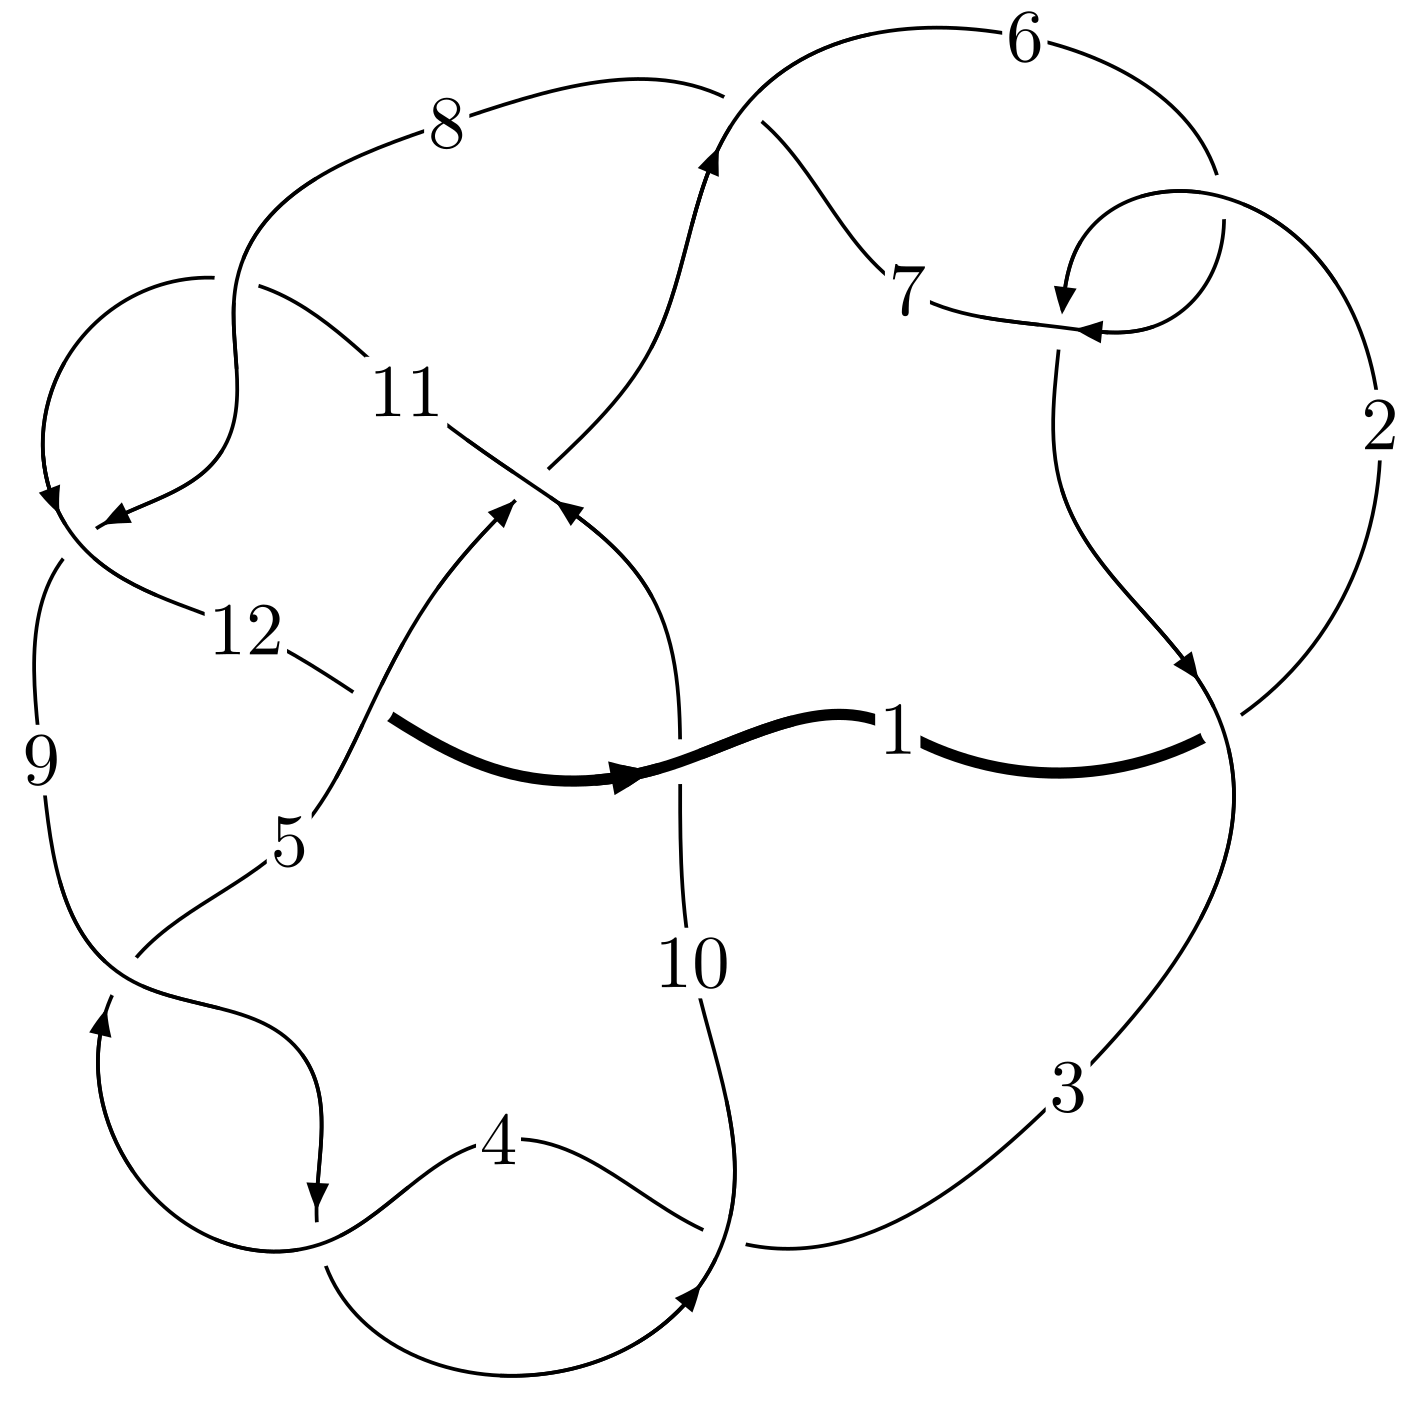
\includegraphics[width=112pt]{../../../GIT/diagram.site/Diagrams/png/1433_12a_0632.png}\\
\ \ \ A knot diagram\footnotemark}&
\allowdisplaybreaks
\textbf{Linearized knot diagam} \\
\cline{2-2}
 &
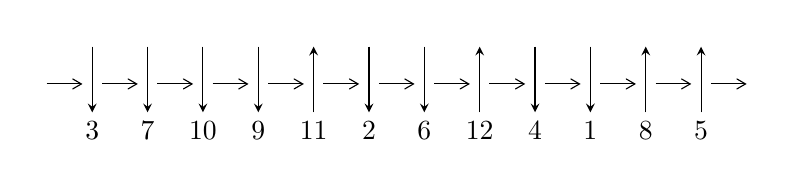
\begin{tikzpicture}[x=20pt, y=17pt]
	% nodes
	\node (C0) at (0, 0) {};
	\node (C1) at (1, 0) {};
	\node (C1U) at (1, +1) {};
	\node (C1D) at (1, -1) {3};

	\node (C2) at (2, 0) {};
	\node (C2U) at (2, +1) {};
	\node (C2D) at (2, -1) {7};

	\node (C3) at (3, 0) {};
	\node (C3U) at (3, +1) {};
	\node (C3D) at (3, -1) {10};

	\node (C4) at (4, 0) {};
	\node (C4U) at (4, +1) {};
	\node (C4D) at (4, -1) {9};

	\node (C5) at (5, 0) {};
	\node (C5U) at (5, +1) {};
	\node (C5D) at (5, -1) {11};

	\node (C6) at (6, 0) {};
	\node (C6U) at (6, +1) {};
	\node (C6D) at (6, -1) {2};

	\node (C7) at (7, 0) {};
	\node (C7U) at (7, +1) {};
	\node (C7D) at (7, -1) {6};

	\node (C8) at (8, 0) {};
	\node (C8U) at (8, +1) {};
	\node (C8D) at (8, -1) {12};

	\node (C9) at (9, 0) {};
	\node (C9U) at (9, +1) {};
	\node (C9D) at (9, -1) {4};

	\node (C10) at (10, 0) {};
	\node (C10U) at (10, +1) {};
	\node (C10D) at (10, -1) {1};

	\node (C11) at (11, 0) {};
	\node (C11U) at (11, +1) {};
	\node (C11D) at (11, -1) {8};

	\node (C12) at (12, 0) {};
	\node (C12U) at (12, +1) {};
	\node (C12D) at (12, -1) {5};
	\node (C13) at (13, 0) {};

	% arrows
	\draw[->,>={angle 60}]
	(C0) edge (C1) (C1) edge (C2) (C2) edge (C3) (C3) edge (C4) (C4) edge (C5) (C5) edge (C6) (C6) edge (C7) (C7) edge (C8) (C8) edge (C9) (C9) edge (C10) (C10) edge (C11) (C11) edge (C12) (C12) edge (C13) ;	\draw[->,>=stealth]
	(C1U) edge (C1D) (C2U) edge (C2D) (C3U) edge (C3D) (C4U) edge (C4D) (C5D) edge (C5U) (C6U) edge (C6D) (C7U) edge (C7D) (C8D) edge (C8U) (C9U) edge (C9D) (C10U) edge (C10D) (C11D) edge (C11U) (C12D) edge (C12U) ;
	\end{tikzpicture} \\
\hhline{~~} \\& 
\textbf{Solving Sequence} \\ \cline{2-2} 
 &
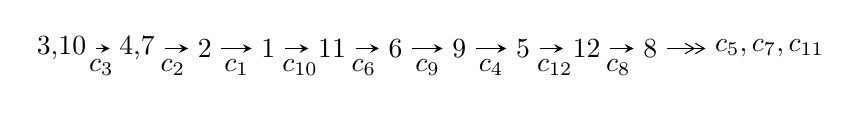
\begin{tikzpicture}[x=23pt, y=7pt]
	% node
	\node (A0) at (-1/8, 0) {3,10};
	\node (A1) at (17/16, 0) {4,7};
	\node (A2) at (17/8, 0) {2};
	\node (A3) at (25/8, 0) {1};
	\node (A4) at (33/8, 0) {11};
	\node (A5) at (41/8, 0) {6};
	\node (A6) at (49/8, 0) {9};
	\node (A7) at (57/8, 0) {5};
	\node (A8) at (65/8, 0) {12};
	\node (A9) at (73/8, 0) {8};
	\node (C1) at (1/2, -1) {$c_{3}$};
	\node (C2) at (13/8, -1) {$c_{2}$};
	\node (C3) at (21/8, -1) {$c_{1}$};
	\node (C4) at (29/8, -1) {$c_{10}$};
	\node (C5) at (37/8, -1) {$c_{6}$};
	\node (C6) at (45/8, -1) {$c_{9}$};
	\node (C7) at (53/8, -1) {$c_{4}$};
	\node (C8) at (61/8, -1) {$c_{12}$};
	\node (C9) at (69/8, -1) {$c_{8}$};
	\node (A10) at (11, 0) {$c_{5},c_{7},c_{11}$};

	% edge
	\draw[->,>=stealth]	
	(A0) edge (A1) (A1) edge (A2) (A2) edge (A3) (A3) edge (A4) (A4) edge (A5) (A5) edge (A6) (A6) edge (A7) (A7) edge (A8) (A8) edge (A9) ;
	\draw[->>,>={angle 60}]	
	(A9) edge (A10);
\end{tikzpicture} \\ 

\end{tabular} \\

\footnotetext{
The image of knot diagram is generated by the software ``\textbf{Draw programme}" developed by Andrew Bartholomew(\url{http://www.layer8.co.uk/maths/draw/index.htm\#Running-draw}), where we modified some parts for our purpose(\url{https://github.com/CATsTAILs/LinksPainter}).
}\phantom \\ \newline 
\centering \textbf{Ideals for irreducible components\footnotemark of $X_{\text{par}}$} 
 
\begin{align*}
I^u_{1}&=\langle 
4.99554\times10^{194} u^{93}+1.87631\times10^{195} u^{92}+\cdots+1.61849\times10^{196} b-2.06106\times10^{197},\\
\phantom{I^u_{1}}&\phantom{= \langle  }3.26120\times10^{197} u^{93}-1.40330\times10^{198} u^{92}+\cdots+3.28554\times10^{198} a+8.49179\times10^{199},\\
\phantom{I^u_{1}}&\phantom{= \langle  }u^{94}- u^{93}+\cdots-167 u-29\rangle \\
I^u_{2}&=\langle 
- u^{12}-7 u^{10}-17 u^8- u^7-15 u^6-4 u^5- u^4-4 u^3+u^2+b-1,\\
\phantom{I^u_{2}}&\phantom{= \langle  }u^{15}+9 u^{13}+31 u^{11}+49 u^9+32 u^7+5 u^5+3 u^3+a+2 u,\;u^{20}+12 u^{18}+\cdots+2 u-1\rangle \\
\\
\end{align*}
\raggedright * 2 irreducible components of $\dim_{\mathbb{C}}=0$, with total 114 representations.\\
\footnotetext{All coefficients of polynomials are rational numbers. But the coefficients are sometimes approximated in decimal forms when there is not enough margin.}
\newpage
\renewcommand{\arraystretch}{1}
\centering \section*{I. $I^u_{1}= \langle 5.00\times10^{194} u^{93}+1.88\times10^{195} u^{92}+\cdots+1.62\times10^{196} b-2.06\times10^{197},\;3.26\times10^{197} u^{93}-1.40\times10^{198} u^{92}+\cdots+3.29\times10^{198} a+8.49\times10^{199},\;u^{94}- u^{93}+\cdots-167 u-29 \rangle$}
\flushleft \textbf{(i) Arc colorings}\\
\begin{tabular}{m{7pt} m{180pt} m{7pt} m{180pt} }
\flushright $a_{3}=$&$\begin{pmatrix}1\\0\end{pmatrix}$ \\
\flushright $a_{10}=$&$\begin{pmatrix}0\\u\end{pmatrix}$ \\
\flushright $a_{4}=$&$\begin{pmatrix}1\\u^2\end{pmatrix}$ \\
\flushright $a_{7}=$&$\begin{pmatrix}-0.0992592 u^{93}+0.427114 u^{92}+\cdots-146.954 u-25.8459\\-0.0308654 u^{93}-0.115930 u^{92}+\cdots+68.0928 u+12.7344\end{pmatrix}$ \\
\flushright $a_{2}=$&$\begin{pmatrix}-0.538405 u^{93}+0.447589 u^{92}+\cdots+266.311 u+35.3348\\0.293053 u^{93}-0.414594 u^{92}+\cdots-26.7401 u+0.924989\end{pmatrix}$ \\
\flushright $a_{1}=$&$\begin{pmatrix}-0.245351 u^{93}+0.0329949 u^{92}+\cdots+239.571 u+36.2598\\0.293053 u^{93}-0.414594 u^{92}+\cdots-26.7401 u+0.924989\end{pmatrix}$ \\
\flushright $a_{11}=$&$\begin{pmatrix}-0.335863 u^{93}+0.0931342 u^{92}+\cdots+376.355 u+59.6146\\0.173090 u^{93}-0.229501 u^{92}+\cdots-103.638 u-13.5395\end{pmatrix}$ \\
\flushright $a_{6}=$&$\begin{pmatrix}-0.973604 u^{93}+1.46961 u^{92}+\cdots-64.1810 u-31.6883\\-0.0839155 u^{93}-0.212165 u^{92}+\cdots+128.396 u+23.5613\end{pmatrix}$ \\
\flushright $a_{9}=$&$\begin{pmatrix}u\\u^3+u\end{pmatrix}$ \\
\flushright $a_{5}=$&$\begin{pmatrix}u^2+1\\u^4+2 u^2\end{pmatrix}$ \\
\flushright $a_{12}=$&$\begin{pmatrix}-0.300038 u^{93}+0.154180 u^{92}+\cdots+196.014 u+27.6672\\0.296675 u^{93}-0.441920 u^{92}+\cdots+7.50288 u+7.58897\end{pmatrix}$ \\
\flushright $a_{8}=$&$\begin{pmatrix}-0.389629 u^{93}-0.0751627 u^{92}+\cdots+300.697 u+46.4877\\-0.0198539 u^{93}+0.200468 u^{92}+\cdots-84.1348 u-15.6577\end{pmatrix}$\\&\end{tabular}
\flushleft \textbf{(ii) Obstruction class $= -1$}\\~\\
\flushleft \textbf{(iii) Cusp Shapes $= -1.16644 u^{93}+1.34986 u^{92}+\cdots+102.241 u-6.06992$}\\~\\
\newpage\renewcommand{\arraystretch}{1}
\flushleft \textbf{(iv) u-Polynomials at the component}\newline \\
\begin{tabular}{m{50pt}|m{274pt}}
Crossings & \hspace{64pt}u-Polynomials at each crossing \\
\hline $$\begin{aligned}c_{1},c_{7}\end{aligned}$$&$\begin{aligned}
&u^{94}+27 u^{93}+\cdots+38 u+1
\end{aligned}$\\
\hline $$\begin{aligned}c_{2},c_{6}\end{aligned}$$&$\begin{aligned}
&u^{94}- u^{93}+\cdots-6 u-1
\end{aligned}$\\
\hline $$\begin{aligned}c_{3},c_{4},c_{9}\end{aligned}$$&$\begin{aligned}
&u^{94}+u^{93}+\cdots+167 u-29
\end{aligned}$\\
\hline $$\begin{aligned}c_{5}\end{aligned}$$&$\begin{aligned}
&u^{94}+u^{93}+\cdots-48236 u-34973
\end{aligned}$\\
\hline $$\begin{aligned}c_{8},c_{11}\end{aligned}$$&$\begin{aligned}
&u^{94}+u^{93}+\cdots+18 u-1
\end{aligned}$\\
\hline $$\begin{aligned}c_{10}\end{aligned}$$&$\begin{aligned}
&u^{94}-15 u^{93}+\cdots-23727557 u+1575181
\end{aligned}$\\
\hline $$\begin{aligned}c_{12}\end{aligned}$$&$\begin{aligned}
&u^{94}-4 u^{93}+\cdots-1684565 u+327443
\end{aligned}$\\
\hline
\end{tabular}\\~\\
\newpage\renewcommand{\arraystretch}{1}
\flushleft \textbf{(v) Riley Polynomials at the component}\newline \\
\begin{tabular}{m{50pt}|m{274pt}}
Crossings & \hspace{64pt}Riley Polynomials at each crossing \\
\hline $$\begin{aligned}c_{1},c_{7}\end{aligned}$$&$\begin{aligned}
&y^{94}+89 y^{93}+\cdots+330 y+1
\end{aligned}$\\
\hline $$\begin{aligned}c_{2},c_{6}\end{aligned}$$&$\begin{aligned}
&y^{94}-27 y^{93}+\cdots-38 y+1
\end{aligned}$\\
\hline $$\begin{aligned}c_{3},c_{4},c_{9}\end{aligned}$$&$\begin{aligned}
&y^{94}+105 y^{93}+\cdots+13233 y+841
\end{aligned}$\\
\hline $$\begin{aligned}c_{5}\end{aligned}$$&$\begin{aligned}
&y^{94}-39 y^{93}+\cdots-42017779234 y+1223110729
\end{aligned}$\\
\hline $$\begin{aligned}c_{8},c_{11}\end{aligned}$$&$\begin{aligned}
&y^{94}-87 y^{93}+\cdots-396 y+1
\end{aligned}$\\
\hline $$\begin{aligned}c_{10}\end{aligned}$$&$\begin{aligned}
&y^{94}+49 y^{93}+\cdots-1793204056987 y+2481195182761
\end{aligned}$\\
\hline $$\begin{aligned}c_{12}\end{aligned}$$&$\begin{aligned}
&y^{94}-46 y^{93}+\cdots-4312336575555 y+107218918249
\end{aligned}$\\
\hline
\end{tabular}\\~\\
\newpage\flushleft \textbf{(vi) Complex Volumes and Cusp Shapes}
$$\begin{array}{c|c|c}  
\text{Solutions to }I^u_{1}& \I (\text{vol} + \sqrt{-1}CS) & \text{Cusp shape}\\
 \hline 
\begin{aligned}
u &= \phantom{-}0.820738 + 0.587626 I \\
a &= \phantom{-}0.440823 - 0.310456 I \\
b &= \phantom{-}0.881355 - 0.271423 I\end{aligned}
 & \phantom{-}0.96039 + 2.29358 I & \phantom{-0.000000 } 0 \\ \hline\begin{aligned}
u &= \phantom{-}0.820738 - 0.587626 I \\
a &= \phantom{-}0.440823 + 0.310456 I \\
b &= \phantom{-}0.881355 + 0.271423 I\end{aligned}
 & \phantom{-}0.96039 - 2.29358 I & \phantom{-0.000000 } 0 \\ \hline\begin{aligned}
u &= \phantom{-}0.718782 + 0.561750 I \\
a &= -0.919278 + 0.814379 I \\
b &= -1.040590 - 0.339974 I\end{aligned}
 & \phantom{-}1.04618 - 7.42407 I & \phantom{-0.000000 } 0 \\ \hline\begin{aligned}
u &= \phantom{-}0.718782 - 0.561750 I \\
a &= -0.919278 - 0.814379 I \\
b &= -1.040590 + 0.339974 I\end{aligned}
 & \phantom{-}1.04618 + 7.42407 I & \phantom{-0.000000 } 0 \\ \hline\begin{aligned}
u &= \phantom{-}0.199350 + 0.836635 I \\
a &= \phantom{-}0.26123 + 1.52112 I \\
b &= -0.781807 - 0.449145 I\end{aligned}
 & \phantom{-}1.25072 - 1.88705 I & \phantom{-0.000000 } 0 \\ \hline\begin{aligned}
u &= \phantom{-}0.199350 - 0.836635 I \\
a &= \phantom{-}0.26123 - 1.52112 I \\
b &= -0.781807 + 0.449145 I\end{aligned}
 & \phantom{-}1.25072 + 1.88705 I & \phantom{-0.000000 } 0 \\ \hline\begin{aligned}
u &= -0.815773 + 0.799685 I \\
a &= -0.606742 - 0.612269 I \\
b &= \phantom{-}0.790217 + 0.879227 I\end{aligned}
 & \phantom{-}9.05964 + 6.09171 I & \phantom{-0.000000 } 0 \\ \hline\begin{aligned}
u &= -0.815773 - 0.799685 I \\
a &= -0.606742 + 0.612269 I \\
b &= \phantom{-}0.790217 - 0.879227 I\end{aligned}
 & \phantom{-}9.05964 - 6.09171 I & \phantom{-0.000000 } 0 \\ \hline\begin{aligned}
u &= -0.271517 + 0.804423 I \\
a &= \phantom{-}0.623640 + 1.187280 I \\
b &= \phantom{-}0.738176 + 0.114073 I\end{aligned}
 & -1.40142 - 0.50343 I & \phantom{-0.000000 } 0 \\ \hline\begin{aligned}
u &= -0.271517 - 0.804423 I \\
a &= \phantom{-}0.623640 - 1.187280 I \\
b &= \phantom{-}0.738176 - 0.114073 I\end{aligned}
 & -1.40142 + 0.50343 I & \phantom{-0.000000 } 0\\
 \hline 
 \end{array}$$\newpage$$\begin{array}{c|c|c}  
\text{Solutions to }I^u_{1}& \I (\text{vol} + \sqrt{-1}CS) & \text{Cusp shape}\\
 \hline 
\begin{aligned}
u &= -0.635589 + 0.559738 I \\
a &= \phantom{-}0.107171 + 0.363611 I \\
b &= -0.877502 - 0.782060 I\end{aligned}
 & \phantom{-}3.53268 - 2.95131 I & \phantom{-0.000000 } 0 \\ \hline\begin{aligned}
u &= -0.635589 - 0.559738 I \\
a &= \phantom{-}0.107171 - 0.363611 I \\
b &= -0.877502 + 0.782060 I\end{aligned}
 & \phantom{-}3.53268 + 2.95131 I & \phantom{-0.000000 } 0 \\ \hline\begin{aligned}
u &= \phantom{-}0.865061 + 0.767344 I \\
a &= \phantom{-}0.51007 - 1.61748 I \\
b &= \phantom{-}0.995348 + 0.801095 I\end{aligned}
 & \phantom{-}8.4200 - 12.3261 I & \phantom{-0.000000 } 0 \\ \hline\begin{aligned}
u &= \phantom{-}0.865061 - 0.767344 I \\
a &= \phantom{-}0.51007 + 1.61748 I \\
b &= \phantom{-}0.995348 - 0.801095 I\end{aligned}
 & \phantom{-}8.4200 + 12.3261 I & \phantom{-0.000000 } 0 \\ \hline\begin{aligned}
u &= -0.077414 + 1.155390 I \\
a &= \phantom{-}0.72139 - 2.10591 I \\
b &= -0.832174 + 0.633495 I\end{aligned}
 & \phantom{-}1.26169 + 2.45313 I & \phantom{-0.000000 } 0 \\ \hline\begin{aligned}
u &= -0.077414 - 1.155390 I \\
a &= \phantom{-}0.72139 + 2.10591 I \\
b &= -0.832174 - 0.633495 I\end{aligned}
 & \phantom{-}1.26169 - 2.45313 I & \phantom{-0.000000 } 0 \\ \hline\begin{aligned}
u &= \phantom{-}0.663089 + 0.467881 I \\
a &= -0.682449 + 1.189480 I \\
b &= -0.897129 - 0.774236 I\end{aligned}
 & \phantom{-}3.46999 - 2.91507 I & \phantom{-0.000000 } 0 \\ \hline\begin{aligned}
u &= \phantom{-}0.663089 - 0.467881 I \\
a &= -0.682449 - 1.189480 I \\
b &= -0.897129 + 0.774236 I\end{aligned}
 & \phantom{-}3.46999 + 2.91507 I & \phantom{-0.000000 } 0 \\ \hline\begin{aligned}
u &= -0.510396 + 0.617981 I \\
a &= -0.006012 + 0.574248 I \\
b &= -0.084323 - 0.749330 I\end{aligned}
 & \phantom{-}4.13181 + 3.70371 I & \phantom{-0.000000 } 0 \\ \hline\begin{aligned}
u &= -0.510396 - 0.617981 I \\
a &= -0.006012 - 0.574248 I \\
b &= -0.084323 + 0.749330 I\end{aligned}
 & \phantom{-}4.13181 - 3.70371 I & \phantom{-0.000000 } 0\\
 \hline 
 \end{array}$$\newpage$$\begin{array}{c|c|c}  
\text{Solutions to }I^u_{1}& \I (\text{vol} + \sqrt{-1}CS) & \text{Cusp shape}\\
 \hline 
\begin{aligned}
u &= \phantom{-}0.586789 + 0.543439 I \\
a &= -0.761137 - 0.077902 I \\
b &= \phantom{-}0.824788 - 0.804257 I\end{aligned}
 & \phantom{-}3.76120 - 1.30617 I & \phantom{-0.000000 } 0 \\ \hline\begin{aligned}
u &= \phantom{-}0.586789 - 0.543439 I \\
a &= -0.761137 + 0.077902 I \\
b &= \phantom{-}0.824788 + 0.804257 I\end{aligned}
 & \phantom{-}3.76120 + 1.30617 I & \phantom{-0.000000 } 0 \\ \hline\begin{aligned}
u &= -0.620759 + 0.498143 I \\
a &= \phantom{-}1.23807 + 1.75646 I \\
b &= \phantom{-}0.943160 - 0.775930 I\end{aligned}
 & \phantom{-}3.39908 + 7.24288 I & \phantom{-0.000000 } 0 \\ \hline\begin{aligned}
u &= -0.620759 - 0.498143 I \\
a &= \phantom{-}1.23807 - 1.75646 I \\
b &= \phantom{-}0.943160 + 0.775930 I\end{aligned}
 & \phantom{-}3.39908 - 7.24288 I & \phantom{-0.000000 } 0 \\ \hline\begin{aligned}
u &= -1.150250 + 0.461742 I \\
a &= -0.335761 - 1.188530 I \\
b &= -0.844510 + 0.830835 I\end{aligned}
 & \phantom{-}7.74170 + 0.30120 I & \phantom{-0.000000 } 0 \\ \hline\begin{aligned}
u &= -1.150250 - 0.461742 I \\
a &= -0.335761 + 1.188530 I \\
b &= -0.844510 - 0.830835 I\end{aligned}
 & \phantom{-}7.74170 - 0.30120 I & \phantom{-0.000000 } 0 \\ \hline\begin{aligned}
u &= \phantom{-}1.142230 + 0.528154 I \\
a &= \phantom{-}0.104805 - 0.704670 I \\
b &= -0.942928 + 0.799373 I\end{aligned}
 & \phantom{-}7.43573 + 5.79082 I & \phantom{-0.000000 } 0 \\ \hline\begin{aligned}
u &= \phantom{-}1.142230 - 0.528154 I \\
a &= \phantom{-}0.104805 + 0.704670 I \\
b &= -0.942928 - 0.799373 I\end{aligned}
 & \phantom{-}7.43573 - 5.79082 I & \phantom{-0.000000 } 0 \\ \hline\begin{aligned}
u &= -0.691704 + 0.069857 I \\
a &= \phantom{-}1.73090 + 0.13000 I \\
b &= \phantom{-}0.185748 - 0.106850 I\end{aligned}
 & \phantom{-}2.85068 - 0.00394 I & \phantom{-}4.77299 + 0. I\phantom{ +0.000000I} \\ \hline\begin{aligned}
u &= -0.691704 - 0.069857 I \\
a &= \phantom{-}1.73090 - 0.13000 I \\
b &= \phantom{-}0.185748 + 0.106850 I\end{aligned}
 & \phantom{-}2.85068 + 0.00394 I & \phantom{-}4.77299 + 0. I\phantom{ +0.000000I}\\
 \hline 
 \end{array}$$\newpage$$\begin{array}{c|c|c}  
\text{Solutions to }I^u_{1}& \I (\text{vol} + \sqrt{-1}CS) & \text{Cusp shape}\\
 \hline 
\begin{aligned}
u &= \phantom{-}0.295863 + 0.613012 I \\
a &= \phantom{-}0.73322 + 1.80671 I \\
b &= -0.809513 - 0.268723 I\end{aligned}
 & \phantom{-}1.13533 - 2.03881 I & \phantom{-0.000000 -}0. + 6.81649 I \\ \hline\begin{aligned}
u &= \phantom{-}0.295863 - 0.613012 I \\
a &= \phantom{-}0.73322 - 1.80671 I \\
b &= -0.809513 + 0.268723 I\end{aligned}
 & \phantom{-}1.13533 + 2.03881 I & \phantom{-0.000000 } 0. - 6.81649 I \\ \hline\begin{aligned}
u &= -0.482695 + 0.333452 I \\
a &= -2.16015 - 0.87654 I \\
b &= -0.914998 + 0.229995 I\end{aligned}
 & -2.63624 + 3.34700 I & -9.84874 - 7.94099 I \\ \hline\begin{aligned}
u &= -0.482695 - 0.333452 I \\
a &= -2.16015 + 0.87654 I \\
b &= -0.914998 - 0.229995 I\end{aligned}
 & -2.63624 - 3.34700 I & -9.84874 + 7.94099 I \\ \hline\begin{aligned}
u &= -0.000183 + 0.585754 I \\
a &= \phantom{-}0.952288 - 0.418442 I \\
b &= -0.755983 + 0.900316 I\end{aligned}
 & \phantom{-}7.97844 + 0.55523 I & \phantom{-}6.56904 - 0.52995 I \\ \hline\begin{aligned}
u &= -0.000183 - 0.585754 I \\
a &= \phantom{-}0.952288 + 0.418442 I \\
b &= -0.755983 - 0.900316 I\end{aligned}
 & \phantom{-}7.97844 - 0.55523 I & \phantom{-}6.56904 + 0.52995 I \\ \hline\begin{aligned}
u &= \phantom{-}0.01950 + 1.42476 I \\
a &= -0.332704 + 0.558349 I \\
b &= -1.049140 - 0.266255 I\end{aligned}
 & \phantom{-}3.04541 - 0.96461 I & \phantom{-0.000000 } 0 \\ \hline\begin{aligned}
u &= \phantom{-}0.01950 - 1.42476 I \\
a &= -0.332704 - 0.558349 I \\
b &= -1.049140 + 0.266255 I\end{aligned}
 & \phantom{-}3.04541 + 0.96461 I & \phantom{-0.000000 } 0 \\ \hline\begin{aligned}
u &= -0.07864 + 1.45458 I \\
a &= \phantom{-}0.64180 - 1.99812 I \\
b &= \phantom{-}0.733749 + 0.278862 I\end{aligned}
 & \phantom{-}8.05807 + 1.16577 I & \phantom{-0.000000 } 0 \\ \hline\begin{aligned}
u &= -0.07864 - 1.45458 I \\
a &= \phantom{-}0.64180 + 1.99812 I \\
b &= \phantom{-}0.733749 - 0.278862 I\end{aligned}
 & \phantom{-}8.05807 - 1.16577 I & \phantom{-0.000000 } 0\\
 \hline 
 \end{array}$$\newpage$$\begin{array}{c|c|c}  
\text{Solutions to }I^u_{1}& \I (\text{vol} + \sqrt{-1}CS) & \text{Cusp shape}\\
 \hline 
\begin{aligned}
u &= -0.11659 + 1.46166 I \\
a &= \phantom{-}0.574879 + 1.242790 I \\
b &= \phantom{-}1.012810 - 0.292217 I\end{aligned}
 & \phantom{-}3.23851 + 5.39050 I & \phantom{-0.000000 } 0 \\ \hline\begin{aligned}
u &= -0.11659 - 1.46166 I \\
a &= \phantom{-}0.574879 - 1.242790 I \\
b &= \phantom{-}1.012810 + 0.292217 I\end{aligned}
 & \phantom{-}3.23851 - 5.39050 I & \phantom{-0.000000 } 0 \\ \hline\begin{aligned}
u &= \phantom{-}0.300332 + 0.436318 I \\
a &= \phantom{-}0.436112 + 0.068253 I \\
b &= \phantom{-}0.002092 + 0.379935 I\end{aligned}
 & -0.137046 - 1.130850 I & -2.15439 + 5.92996 I \\ \hline\begin{aligned}
u &= \phantom{-}0.300332 - 0.436318 I \\
a &= \phantom{-}0.436112 - 0.068253 I \\
b &= \phantom{-}0.002092 - 0.379935 I\end{aligned}
 & -0.137046 + 1.130850 I & -2.15439 - 5.92996 I \\ \hline\begin{aligned}
u &= -0.051296 + 0.521935 I \\
a &= -2.87878 - 1.09502 I \\
b &= \phantom{-}0.931068 + 0.788334 I\end{aligned}
 & \phantom{-}7.18856 - 5.21612 I & \phantom{-}6.82948 + 5.47677 I \\ \hline\begin{aligned}
u &= -0.051296 - 0.521935 I \\
a &= -2.87878 + 1.09502 I \\
b &= \phantom{-}0.931068 - 0.788334 I\end{aligned}
 & \phantom{-}7.18856 + 5.21612 I & \phantom{-}6.82948 - 5.47677 I \\ \hline\begin{aligned}
u &= -0.085886 + 0.513350 I \\
a &= -0.74177 - 2.07353 I \\
b &= -1.021080 + 0.802754 I\end{aligned}
 & \phantom{-}7.16169 + 5.74033 I & \phantom{-}4.97732 - 6.13962 I \\ \hline\begin{aligned}
u &= -0.085886 - 0.513350 I \\
a &= -0.74177 + 2.07353 I \\
b &= -1.021080 - 0.802754 I\end{aligned}
 & \phantom{-}7.16169 - 5.74033 I & \phantom{-}4.97732 + 6.13962 I \\ \hline\begin{aligned}
u &= \phantom{-}0.378489 + 0.334490 I \\
a &= \phantom{-}0.711457 + 0.594518 I \\
b &= \phantom{-}1.135660 - 0.192281 I\end{aligned}
 & \phantom{-}0.066201 - 0.543447 I & -1.68971 + 10.03219 I \\ \hline\begin{aligned}
u &= \phantom{-}0.378489 - 0.334490 I \\
a &= \phantom{-}0.711457 - 0.594518 I \\
b &= \phantom{-}1.135660 + 0.192281 I\end{aligned}
 & \phantom{-}0.066201 + 0.543447 I & -1.68971 - 10.03219 I\\
 \hline 
 \end{array}$$\newpage$$\begin{array}{c|c|c}  
\text{Solutions to }I^u_{1}& \I (\text{vol} + \sqrt{-1}CS) & \text{Cusp shape}\\
 \hline 
\begin{aligned}
u &= \phantom{-}0.04902 + 1.50808 I \\
a &= -0.205130 + 0.843593 I \\
b &= \phantom{-}0.004830 - 0.661595 I\end{aligned}
 & \phantom{-}6.35559 - 2.20338 I & \phantom{-0.000000 } 0 \\ \hline\begin{aligned}
u &= \phantom{-}0.04902 - 1.50808 I \\
a &= -0.205130 - 0.843593 I \\
b &= \phantom{-}0.004830 + 0.661595 I\end{aligned}
 & \phantom{-}6.35559 + 2.20338 I & \phantom{-0.000000 } 0 \\ \hline\begin{aligned}
u &= \phantom{-}0.09006 + 1.50644 I \\
a &= \phantom{-}0.177929 - 0.400798 I \\
b &= -1.312220 + 0.208394 I\end{aligned}
 & \phantom{-}6.32186 - 2.06708 I & \phantom{-0.000000 } 0 \\ \hline\begin{aligned}
u &= \phantom{-}0.09006 - 1.50644 I \\
a &= \phantom{-}0.177929 + 0.400798 I \\
b &= -1.312220 - 0.208394 I\end{aligned}
 & \phantom{-}6.32186 + 2.06708 I & \phantom{-0.000000 } 0 \\ \hline\begin{aligned}
u &= -0.28507 + 1.50115 I \\
a &= -0.925190 - 0.903580 I \\
b &= -0.729288 + 0.331136 I\end{aligned}
 & \phantom{-}8.32963 + 4.12866 I & \phantom{-0.000000 } 0 \\ \hline\begin{aligned}
u &= -0.28507 - 1.50115 I \\
a &= -0.925190 + 0.903580 I \\
b &= -0.729288 - 0.331136 I\end{aligned}
 & \phantom{-}8.32963 - 4.12866 I & \phantom{-0.000000 } 0 \\ \hline\begin{aligned}
u &= -0.17857 + 1.52580 I \\
a &= -0.19993 - 2.38320 I \\
b &= -0.981214 + 0.788797 I\end{aligned}
 & \phantom{-}10.0840 + 10.0843 I & \phantom{-0.000000 } 0 \\ \hline\begin{aligned}
u &= -0.17857 - 1.52580 I \\
a &= -0.19993 + 2.38320 I \\
b &= -0.981214 - 0.788797 I\end{aligned}
 & \phantom{-}10.0840 - 10.0843 I & \phantom{-0.000000 } 0 \\ \hline\begin{aligned}
u &= \phantom{-}0.01876 + 1.53818 I \\
a &= \phantom{-}0.50168 + 2.75318 I \\
b &= -0.906877 - 0.816322 I\end{aligned}
 & \phantom{-}14.2850 - 1.0715 I & \phantom{-0.000000 } 0 \\ \hline\begin{aligned}
u &= \phantom{-}0.01876 - 1.53818 I \\
a &= \phantom{-}0.50168 - 2.75318 I \\
b &= -0.906877 + 0.816322 I\end{aligned}
 & \phantom{-}14.2850 + 1.0715 I & \phantom{-0.000000 } 0\\
 \hline 
 \end{array}$$\newpage$$\begin{array}{c|c|c}  
\text{Solutions to }I^u_{1}& \I (\text{vol} + \sqrt{-1}CS) & \text{Cusp shape}\\
 \hline 
\begin{aligned}
u &= \phantom{-}0.16297 + 1.53875 I \\
a &= \phantom{-}1.35628 - 0.85930 I \\
b &= -0.793481 + 0.850541 I\end{aligned}
 & \phantom{-}10.66380 - 3.97201 I & \phantom{-0.000000 } 0 \\ \hline\begin{aligned}
u &= \phantom{-}0.16297 - 1.53875 I \\
a &= \phantom{-}1.35628 + 0.85930 I \\
b &= -0.793481 - 0.850541 I\end{aligned}
 & \phantom{-}10.66380 + 3.97201 I & \phantom{-0.000000 } 0 \\ \hline\begin{aligned}
u &= \phantom{-}0.056940 + 0.447762 I \\
a &= \phantom{-}0.07733 - 4.59205 I \\
b &= \phantom{-}0.848197 + 0.813608 I\end{aligned}
 & \phantom{-}7.44639 - 0.78804 I & \phantom{-}7.86918 - 0.12351 I \\ \hline\begin{aligned}
u &= \phantom{-}0.056940 - 0.447762 I \\
a &= \phantom{-}0.07733 + 4.59205 I \\
b &= \phantom{-}0.848197 - 0.813608 I\end{aligned}
 & \phantom{-}7.44639 + 0.78804 I & \phantom{-}7.86918 + 0.12351 I \\ \hline\begin{aligned}
u &= -0.02446 + 1.55322 I \\
a &= -0.37266 + 1.86761 I \\
b &= \phantom{-}1.087400 - 0.843941 I\end{aligned}
 & \phantom{-}14.2681 + 6.1381 I & \phantom{-0.000000 } 0 \\ \hline\begin{aligned}
u &= -0.02446 - 1.55322 I \\
a &= -0.37266 - 1.86761 I \\
b &= \phantom{-}1.087400 + 0.843941 I\end{aligned}
 & \phantom{-}14.2681 - 6.1381 I & \phantom{-0.000000 } 0 \\ \hline\begin{aligned}
u &= \phantom{-}0.20649 + 1.53975 I \\
a &= -0.15588 - 1.89554 I \\
b &= \phantom{-}0.994097 + 0.801925 I\end{aligned}
 & \phantom{-}10.13680 - 6.11038 I & \phantom{-0.000000 } 0 \\ \hline\begin{aligned}
u &= \phantom{-}0.20649 - 1.53975 I \\
a &= -0.15588 + 1.89554 I \\
b &= \phantom{-}0.994097 - 0.801925 I\end{aligned}
 & \phantom{-}10.13680 + 6.11038 I & \phantom{-0.000000 } 0 \\ \hline\begin{aligned}
u &= -0.00658 + 1.55610 I \\
a &= \phantom{-}1.70159 + 1.60544 I \\
b &= -0.888262 - 0.822282 I\end{aligned}
 & \phantom{-}14.3430 - 5.0485 I & \phantom{-0.000000 } 0 \\ \hline\begin{aligned}
u &= -0.00658 - 1.55610 I \\
a &= \phantom{-}1.70159 - 1.60544 I \\
b &= -0.888262 + 0.822282 I\end{aligned}
 & \phantom{-}14.3430 + 5.0485 I & \phantom{-0.000000 } 0\\
 \hline 
 \end{array}$$\newpage$$\begin{array}{c|c|c}  
\text{Solutions to }I^u_{1}& \I (\text{vol} + \sqrt{-1}CS) & \text{Cusp shape}\\
 \hline 
\begin{aligned}
u &= \phantom{-}0.21724 + 1.54298 I \\
a &= \phantom{-}0.111391 - 1.183470 I \\
b &= \phantom{-}1.142230 + 0.409534 I\end{aligned}
 & \phantom{-}7.96596 - 10.79960 I & \phantom{-0.000000 } 0 \\ \hline\begin{aligned}
u &= \phantom{-}0.21724 - 1.54298 I \\
a &= \phantom{-}0.111391 + 1.183470 I \\
b &= \phantom{-}1.142230 - 0.409534 I\end{aligned}
 & \phantom{-}7.96596 + 10.79960 I & \phantom{-0.000000 } 0 \\ \hline\begin{aligned}
u &= \phantom{-}0.08889 + 1.55890 I \\
a &= -1.06467 - 1.11922 I \\
b &= \phantom{-}0.633541 + 0.264130 I\end{aligned}
 & \phantom{-}8.41592 - 3.43999 I & \phantom{-0.000000 } 0 \\ \hline\begin{aligned}
u &= \phantom{-}0.08889 - 1.55890 I \\
a &= -1.06467 + 1.11922 I \\
b &= \phantom{-}0.633541 - 0.264130 I\end{aligned}
 & \phantom{-}8.41592 + 3.43999 I & \phantom{-0.000000 } 0 \\ \hline\begin{aligned}
u &= \phantom{-}0.435116\phantom{ +0.000000I} \\
a &= \phantom{-}1.19176\phantom{ +0.000000I} \\
b &= \phantom{-}0.785407\phantom{ +0.000000I}\end{aligned}
 & -1.15748\phantom{ +0.000000I} & -8.95110\phantom{ +0.000000I} \\ \hline\begin{aligned}
u &= -0.00748 + 1.56799 I \\
a &= -0.84679 + 1.38761 I \\
b &= \phantom{-}0.737098 - 1.016210 I\end{aligned}
 & \phantom{-}15.3759 + 0.6273 I & \phantom{-0.000000 } 0 \\ \hline\begin{aligned}
u &= -0.00748 - 1.56799 I \\
a &= -0.84679 - 1.38761 I \\
b &= \phantom{-}0.737098 + 1.016210 I\end{aligned}
 & \phantom{-}15.3759 - 0.6273 I & \phantom{-0.000000 } 0 \\ \hline\begin{aligned}
u &= -0.14946 + 1.56329 I \\
a &= -0.237754 - 1.199410 I \\
b &= \phantom{-}0.126842 + 0.945947 I\end{aligned}
 & \phantom{-}11.42390 + 6.11641 I & \phantom{-0.000000 } 0 \\ \hline\begin{aligned}
u &= -0.14946 - 1.56329 I \\
a &= -0.237754 + 1.199410 I \\
b &= \phantom{-}0.126842 - 0.945947 I\end{aligned}
 & \phantom{-}11.42390 - 6.11641 I & \phantom{-0.000000 } 0 \\ \hline\begin{aligned}
u &= -0.15739 + 1.56991 I \\
a &= -0.87556 - 1.20713 I \\
b &= \phantom{-}0.791167 + 0.873078 I\end{aligned}
 & \phantom{-}10.76480 - 0.11126 I & \phantom{-0.000000 } 0\\
 \hline 
 \end{array}$$\newpage$$\begin{array}{c|c|c}  
\text{Solutions to }I^u_{1}& \I (\text{vol} + \sqrt{-1}CS) & \text{Cusp shape}\\
 \hline 
\begin{aligned}
u &= -0.15739 - 1.56991 I \\
a &= -0.87556 + 1.20713 I \\
b &= \phantom{-}0.791167 - 0.873078 I\end{aligned}
 & \phantom{-}10.76480 + 0.11126 I & \phantom{-0.000000 } 0 \\ \hline\begin{aligned}
u &= \phantom{-}0.18660 + 1.62275 I \\
a &= \phantom{-}0.301803 - 0.266790 I \\
b &= -0.627194 + 0.322697 I\end{aligned}
 & \phantom{-}8.67469 - 1.47071 I & \phantom{-0.000000 } 0 \\ \hline\begin{aligned}
u &= \phantom{-}0.18660 - 1.62275 I \\
a &= \phantom{-}0.301803 + 0.266790 I \\
b &= -0.627194 - 0.322697 I\end{aligned}
 & \phantom{-}8.67469 + 1.47071 I & \phantom{-0.000000 } 0 \\ \hline\begin{aligned}
u &= -0.24840 + 1.63617 I \\
a &= \phantom{-}1.08887 + 1.12188 I \\
b &= -0.782845 - 0.940726 I\end{aligned}
 & \phantom{-}17.1334 + 10.0750 I & \phantom{-0.000000 } 0 \\ \hline\begin{aligned}
u &= -0.24840 - 1.63617 I \\
a &= \phantom{-}1.08887 - 1.12188 I \\
b &= -0.782845 + 0.940726 I\end{aligned}
 & \phantom{-}17.1334 - 10.0750 I & \phantom{-0.000000 } 0 \\ \hline\begin{aligned}
u &= \phantom{-}0.27031 + 1.63345 I \\
a &= \phantom{-}0.04427 + 2.10192 I \\
b &= -1.030210 - 0.824005 I\end{aligned}
 & \phantom{-}16.3449 - 16.5646 I & \phantom{-0.000000 } 0 \\ \hline\begin{aligned}
u &= \phantom{-}0.27031 - 1.63345 I \\
a &= \phantom{-}0.04427 - 2.10192 I \\
b &= -1.030210 + 0.824005 I\end{aligned}
 & \phantom{-}16.3449 + 16.5646 I & \phantom{-0.000000 } 0 \\ \hline\begin{aligned}
u &= -0.289565\phantom{ +0.000000I} \\
a &= \phantom{-}6.60678\phantom{ +0.000000I} \\
b &= -0.406278\phantom{ +0.000000I}\end{aligned}
 & \phantom{-}2.74746\phantom{ +0.000000I} & \phantom{-}8.96970\phantom{ +0.000000I} \\ \hline\begin{aligned}
u &= -0.234229 + 0.135956 I \\
a &= \phantom{-}3.16603 - 0.77183 I \\
b &= \phantom{-}0.872341 + 0.394830 I\end{aligned}
 & -1.88761 - 1.44450 I & -11.71074 + 3.98998 I \\ \hline\begin{aligned}
u &= -0.234229 - 0.135956 I \\
a &= \phantom{-}3.16603 + 0.77183 I \\
b &= \phantom{-}0.872341 - 0.394830 I\end{aligned}
 & -1.88761 + 1.44450 I & -11.71074 - 3.98998 I\\
 \hline 
 \end{array}$$\newpage$$\begin{array}{c|c|c}  
\text{Solutions to }I^u_{1}& \I (\text{vol} + \sqrt{-1}CS) & \text{Cusp shape}\\
 \hline 
\begin{aligned}
u &= -0.38422 + 1.68637 I \\
a &= -0.06395 + 1.90894 I \\
b &= \phantom{-}0.909420 - 0.826421 I\end{aligned}
 & \phantom{-}14.9021 + 6.2030 I & \phantom{-0.000000 } 0 \\ \hline\begin{aligned}
u &= -0.38422 - 1.68637 I \\
a &= -0.06395 - 1.90894 I \\
b &= \phantom{-}0.909420 + 0.826421 I\end{aligned}
 & \phantom{-}14.9021 - 6.2030 I & \phantom{-0.000000 } 0 \\ \hline\begin{aligned}
u &= \phantom{-}0.35426 + 1.70934 I \\
a &= -0.87648 + 1.13190 I \\
b &= \phantom{-}0.892376 - 0.832193 I\end{aligned}
 & \phantom{-}14.9552 - 0.0207 I & \phantom{-0.000000 } 0 \\ \hline\begin{aligned}
u &= \phantom{-}0.35426 - 1.70934 I \\
a &= -0.87648 - 1.13190 I \\
b &= \phantom{-}0.892376 + 0.832193 I\end{aligned}
 & \phantom{-}14.9552 + 0.0207 I & \phantom{-0.000000 } 0\\
 \hline 
 \end{array}$$\newpage\newpage\renewcommand{\arraystretch}{1}
\centering \section*{II. $I^u_{2}= \langle - u^{12}-7 u^{10}+\cdots+b-1,\;u^{15}+9 u^{13}+\cdots+a+2 u,\;u^{20}+12 u^{18}+\cdots+2 u-1 \rangle$}
\flushleft \textbf{(i) Arc colorings}\\
\begin{tabular}{m{7pt} m{180pt} m{7pt} m{180pt} }
\flushright $a_{3}=$&$\begin{pmatrix}1\\0\end{pmatrix}$ \\
\flushright $a_{10}=$&$\begin{pmatrix}0\\u\end{pmatrix}$ \\
\flushright $a_{4}=$&$\begin{pmatrix}1\\u^2\end{pmatrix}$ \\
\flushright $a_{7}=$&$\begin{pmatrix}- u^{15}-9 u^{13}-31 u^{11}-49 u^9-32 u^7-5 u^5-3 u^3-2 u\\u^{12}+7 u^{10}+17 u^8+u^7+15 u^6+4 u^5+u^4+4 u^3- u^2+1\end{pmatrix}$ \\
\flushright $a_{2}=$&$\begin{pmatrix}u^{19}+11 u^{17}+\cdots+2 u+1\\- u^{19}-11 u^{17}+\cdots-4 u^3-1\end{pmatrix}$ \\
\flushright $a_{1}=$&$\begin{pmatrix}u^3+2 u\\- u^{19}-11 u^{17}+\cdots-4 u^3-1\end{pmatrix}$ \\
\flushright $a_{11}=$&$\begin{pmatrix}- u^7-4 u^5-4 u^3\\- u^9-5 u^7-7 u^5- u^3+2 u\end{pmatrix}$ \\
\flushright $a_{6}=$&$\begin{pmatrix}u^{10}+6 u^8+12 u^6+8 u^4+u^2+1\\u^{12}+7 u^{10}+17 u^8+15 u^6+u^4-2 u^2\end{pmatrix}$ \\
\flushright $a_{9}=$&$\begin{pmatrix}u\\u^3+u\end{pmatrix}$ \\
\flushright $a_{5}=$&$\begin{pmatrix}u^2+1\\u^4+2 u^2\end{pmatrix}$ \\
\flushright $a_{12}=$&$\begin{pmatrix}u^{19}+11 u^{17}+\cdots+3 u+1\\- u^{19}-11 u^{17}+\cdots+u-1\end{pmatrix}$ \\
\flushright $a_{8}=$&$\begin{pmatrix}- u^{17}-10 u^{15}+\cdots-3 u-1\\u^{17}+10 u^{15}+\cdots+u+1\end{pmatrix}$\\&\end{tabular}
\flushleft \textbf{(ii) Obstruction class $= 1$}\\~\\
\flushleft \textbf{(iii) Cusp Shapes $= 4 u^{19}+47 u^{17}-2 u^{16}+225 u^{15}-16 u^{14}+553 u^{13}-42 u^{12}+709 u^{11}-24 u^{10}+398 u^9+59 u^8+23 u^7+72 u^6+u^4+36 u^3-5 u^2+2 u+1$}\\~\\
\newpage\renewcommand{\arraystretch}{1}
\flushleft \textbf{(iv) u-Polynomials at the component}\newline \\
\begin{tabular}{m{50pt}|m{274pt}}
Crossings & \hspace{64pt}u-Polynomials at each crossing \\
\hline $$\begin{aligned}c_{1}\end{aligned}$$&$\begin{aligned}
&u^{20}-8 u^{19}+\cdots-15 u+1
\end{aligned}$\\
\hline $$\begin{aligned}c_{2}\end{aligned}$$&$\begin{aligned}
&u^{20}-4 u^{18}+\cdots+u+1
\end{aligned}$\\
\hline $$\begin{aligned}c_{3},c_{4}\end{aligned}$$&$\begin{aligned}
&u^{20}+12 u^{18}+\cdots+2 u-1
\end{aligned}$\\
\hline $$\begin{aligned}c_{5}\end{aligned}$$&$\begin{aligned}
&u^{20}-2 u^{18}+\cdots- u-1
\end{aligned}$\\
\hline $$\begin{aligned}c_{6}\end{aligned}$$&$\begin{aligned}
&u^{20}-4 u^{18}+\cdots- u+1
\end{aligned}$\\
\hline $$\begin{aligned}c_{7}\end{aligned}$$&$\begin{aligned}
&u^{20}+8 u^{19}+\cdots+15 u+1
\end{aligned}$\\
\hline $$\begin{aligned}c_{8}\end{aligned}$$&$\begin{aligned}
&u^{20}-4 u^{19}+\cdots+5 u+1
\end{aligned}$\\
\hline $$\begin{aligned}c_{9}\end{aligned}$$&$\begin{aligned}
&u^{20}+12 u^{18}+\cdots-2 u-1
\end{aligned}$\\
\hline $$\begin{aligned}c_{10}\end{aligned}$$&$\begin{aligned}
&u^{20}+4 u^{19}+\cdots+6 u+1
\end{aligned}$\\
\hline $$\begin{aligned}c_{11}\end{aligned}$$&$\begin{aligned}
&u^{20}+4 u^{19}+\cdots-5 u+1
\end{aligned}$\\
\hline $$\begin{aligned}c_{12}\end{aligned}$$&$\begin{aligned}
&u^{20}+u^{19}+\cdots+2 u^2-1
\end{aligned}$\\
\hline
\end{tabular}\\~\\
\newpage\renewcommand{\arraystretch}{1}
\flushleft \textbf{(v) Riley Polynomials at the component}\newline \\
\begin{tabular}{m{50pt}|m{274pt}}
Crossings & \hspace{64pt}Riley Polynomials at each crossing \\
\hline $$\begin{aligned}c_{1},c_{7}\end{aligned}$$&$\begin{aligned}
&y^{20}+16 y^{19}+\cdots-19 y+1
\end{aligned}$\\
\hline $$\begin{aligned}c_{2},c_{6}\end{aligned}$$&$\begin{aligned}
&y^{20}-8 y^{19}+\cdots-15 y+1
\end{aligned}$\\
\hline $$\begin{aligned}c_{3},c_{4},c_{9}\end{aligned}$$&$\begin{aligned}
&y^{20}+24 y^{19}+\cdots-8 y+1
\end{aligned}$\\
\hline $$\begin{aligned}c_{5}\end{aligned}$$&$\begin{aligned}
&y^{20}-4 y^{19}+\cdots-7 y+1
\end{aligned}$\\
\hline $$\begin{aligned}c_{8},c_{11}\end{aligned}$$&$\begin{aligned}
&y^{20}-24 y^{19}+\cdots+39 y+1
\end{aligned}$\\
\hline $$\begin{aligned}c_{10}\end{aligned}$$&$\begin{aligned}
&y^{20}+4 y^{19}+\cdots-20 y+1
\end{aligned}$\\
\hline $$\begin{aligned}c_{12}\end{aligned}$$&$\begin{aligned}
&y^{20}-7 y^{19}+\cdots-4 y+1
\end{aligned}$\\
\hline
\end{tabular}\\~\\
\newpage\flushleft \textbf{(vi) Complex Volumes and Cusp Shapes}
$$\begin{array}{c|c|c}  
\text{Solutions to }I^u_{2}& \I (\text{vol} + \sqrt{-1}CS) & \text{Cusp shape}\\
 \hline 
\begin{aligned}
u &= \phantom{-}0.082617 + 0.972592 I \\
a &= \phantom{-}0.46585 + 2.01695 I \\
b &= -0.820647 - 0.519052 I\end{aligned}
 & \phantom{-}0.07220 - 2.08153 I & -5.27988 + 3.56850 I \\ \hline\begin{aligned}
u &= \phantom{-}0.082617 - 0.972592 I \\
a &= \phantom{-}0.46585 - 2.01695 I \\
b &= -0.820647 + 0.519052 I\end{aligned}
 & \phantom{-}0.07220 + 2.08153 I & -5.27988 - 3.56850 I \\ \hline\begin{aligned}
u &= \phantom{-}0.145657 + 0.667229 I \\
a &= \phantom{-}0.668097 - 0.491145 I \\
b &= \phantom{-}0.787890 - 0.308801 I\end{aligned}
 & -0.99868 + 1.31531 I & -1.48801 - 4.97789 I \\ \hline\begin{aligned}
u &= \phantom{-}0.145657 - 0.667229 I \\
a &= \phantom{-}0.668097 + 0.491145 I \\
b &= \phantom{-}0.787890 + 0.308801 I\end{aligned}
 & -0.99868 - 1.31531 I & -1.48801 + 4.97789 I \\ \hline\begin{aligned}
u &= -0.596499 + 0.244913 I \\
a &= -1.02878 - 1.75372 I \\
b &= -0.826291 + 0.815126 I\end{aligned}
 & \phantom{-}6.42751 + 1.06605 I & -1.05015 - 2.88825 I \\ \hline\begin{aligned}
u &= -0.596499 - 0.244913 I \\
a &= -1.02878 + 1.75372 I \\
b &= -0.826291 - 0.815126 I\end{aligned}
 & \phantom{-}6.42751 - 1.06605 I & -1.05015 + 2.88825 I \\ \hline\begin{aligned}
u &= \phantom{-}0.563183 + 0.309037 I \\
a &= \phantom{-}0.586211 - 0.158353 I \\
b &= -0.951603 + 0.784592 I\end{aligned}
 & \phantom{-}6.04203 + 4.93414 I & -1.54489 - 2.49382 I \\ \hline\begin{aligned}
u &= \phantom{-}0.563183 - 0.309037 I \\
a &= \phantom{-}0.586211 + 0.158353 I \\
b &= -0.951603 - 0.784592 I\end{aligned}
 & \phantom{-}6.04203 - 4.93414 I & -1.54489 + 2.49382 I \\ \hline\begin{aligned}
u &= -0.594374\phantom{ +0.000000I} \\
a &= \phantom{-}3.59409\phantom{ +0.000000I} \\
b &= \phantom{-}0.575317\phantom{ +0.000000I}\end{aligned}
 & \phantom{-}2.33297\phantom{ +0.000000I} & -12.8660\phantom{ +0.000000I} \\ \hline\begin{aligned}
u &= \phantom{-}0.21953 + 1.44872 I \\
a &= \phantom{-}0.19440 - 1.71239 I \\
b &= \phantom{-}1.007370 + 0.750824 I\end{aligned}
 & \phantom{-}10.38950 - 7.88778 I & \phantom{-}3.85457 + 6.32689 I\\
 \hline 
 \end{array}$$\newpage$$\begin{array}{c|c|c}  
\text{Solutions to }I^u_{2}& \I (\text{vol} + \sqrt{-1}CS) & \text{Cusp shape}\\
 \hline 
\begin{aligned}
u &= \phantom{-}0.21953 - 1.44872 I \\
a &= \phantom{-}0.19440 + 1.71239 I \\
b &= \phantom{-}1.007370 - 0.750824 I\end{aligned}
 & \phantom{-}10.38950 + 7.88778 I & \phantom{-}3.85457 - 6.32689 I \\ \hline\begin{aligned}
u &= \phantom{-}0.09667 + 1.47937 I \\
a &= -0.058612 - 0.469253 I \\
b &= -1.152870 + 0.128392 I\end{aligned}
 & \phantom{-}5.72078 - 1.52942 I & -2.50362 - 1.38490 I \\ \hline\begin{aligned}
u &= \phantom{-}0.09667 - 1.47937 I \\
a &= -0.058612 + 0.469253 I \\
b &= -1.152870 - 0.128392 I\end{aligned}
 & \phantom{-}5.72078 + 1.52942 I & -2.50362 + 1.38490 I \\ \hline\begin{aligned}
u &= -0.21415 + 1.48809 I \\
a &= -0.663577 - 0.745150 I \\
b &= \phantom{-}0.749243 + 0.805642 I\end{aligned}
 & \phantom{-}11.18290 + 2.01192 I & \phantom{-}5.40727 - 0.66728 I \\ \hline\begin{aligned}
u &= -0.21415 - 1.48809 I \\
a &= -0.663577 + 0.745150 I \\
b &= \phantom{-}0.749243 - 0.805642 I\end{aligned}
 & \phantom{-}11.18290 - 2.01192 I & \phantom{-}5.40727 + 0.66728 I \\ \hline\begin{aligned}
u &= -0.14597 + 1.55577 I \\
a &= \phantom{-}0.339045 - 1.226810 I \\
b &= -0.524487 + 0.125129 I\end{aligned}
 & \phantom{-}8.32194 + 2.75801 I & \phantom{-}0.496027 + 0.458149 I \\ \hline\begin{aligned}
u &= -0.14597 - 1.55577 I \\
a &= \phantom{-}0.339045 + 1.226810 I \\
b &= -0.524487 - 0.125129 I\end{aligned}
 & \phantom{-}8.32194 - 2.75801 I & \phantom{-}0.496027 - 0.458149 I \\ \hline\begin{aligned}
u &= -0.01754 + 1.60857 I \\
a &= -0.90265 + 1.90473 I \\
b &= \phantom{-}0.903263 - 0.859516 I\end{aligned}
 & \phantom{-}14.0387 + 3.1794 I & \phantom{-}4.78161 - 2.41137 I \\ \hline\begin{aligned}
u &= -0.01754 - 1.60857 I \\
a &= -0.90265 - 1.90473 I \\
b &= \phantom{-}0.903263 + 0.859516 I\end{aligned}
 & \phantom{-}14.0387 - 3.1794 I & \phantom{-}4.78161 + 2.41137 I \\ \hline\begin{aligned}
u &= \phantom{-}0.327398\phantom{ +0.000000I} \\
a &= -0.794054\phantom{ +0.000000I} \\
b &= \phantom{-}1.08094\phantom{ +0.000000I}\end{aligned}
 & \phantom{-}0.288303\phantom{ +0.000000I} & \phantom{-}2.51980\phantom{ +0.000000I}\\
 \hline 
 \end{array}$$\newpage
\newpage\renewcommand{\arraystretch}{1}
\centering \section*{ III. u-Polynomials}
\begin{tabular}{m{50pt}|m{274pt}}
Crossings & \hspace{64pt}u-Polynomials at each crossing \\
\hline $$\begin{aligned}c_{1}\end{aligned}$$&$\begin{aligned}
&(u^{20}-8 u^{19}+\cdots-15 u+1)(u^{94}+27 u^{93}+\cdots+38 u+1)
\end{aligned}$\\
\hline $$\begin{aligned}c_{2}\end{aligned}$$&$\begin{aligned}
&(u^{20}-4 u^{18}+\cdots+u+1)(u^{94}- u^{93}+\cdots-6 u-1)
\end{aligned}$\\
\hline $$\begin{aligned}c_{3},c_{4}\end{aligned}$$&$\begin{aligned}
&(u^{20}+12 u^{18}+\cdots+2 u-1)(u^{94}+u^{93}+\cdots+167 u-29)
\end{aligned}$\\
\hline $$\begin{aligned}c_{5}\end{aligned}$$&$\begin{aligned}
&(u^{20}-2 u^{18}+\cdots- u-1)(u^{94}+u^{93}+\cdots-48236 u-34973)
\end{aligned}$\\
\hline $$\begin{aligned}c_{6}\end{aligned}$$&$\begin{aligned}
&(u^{20}-4 u^{18}+\cdots- u+1)(u^{94}- u^{93}+\cdots-6 u-1)
\end{aligned}$\\
\hline $$\begin{aligned}c_{7}\end{aligned}$$&$\begin{aligned}
&(u^{20}+8 u^{19}+\cdots+15 u+1)(u^{94}+27 u^{93}+\cdots+38 u+1)
\end{aligned}$\\
\hline $$\begin{aligned}c_{8}\end{aligned}$$&$\begin{aligned}
&(u^{20}-4 u^{19}+\cdots+5 u+1)(u^{94}+u^{93}+\cdots+18 u-1)
\end{aligned}$\\
\hline $$\begin{aligned}c_{9}\end{aligned}$$&$\begin{aligned}
&(u^{20}+12 u^{18}+\cdots-2 u-1)(u^{94}+u^{93}+\cdots+167 u-29)
\end{aligned}$\\
\hline $$\begin{aligned}c_{10}\end{aligned}$$&$\begin{aligned}
&(u^{20}+4 u^{19}+\cdots+6 u+1)\\
&\cdot(u^{94}-15 u^{93}+\cdots-23727557 u+1575181)
\end{aligned}$\\
\hline $$\begin{aligned}c_{11}\end{aligned}$$&$\begin{aligned}
&(u^{20}+4 u^{19}+\cdots-5 u+1)(u^{94}+u^{93}+\cdots+18 u-1)
\end{aligned}$\\
\hline $$\begin{aligned}c_{12}\end{aligned}$$&$\begin{aligned}
&(u^{20}+u^{19}+\cdots+2 u^2-1)(u^{94}-4 u^{93}+\cdots-1684565 u+327443)
\end{aligned}$\\
\hline
\end{tabular}\newpage\renewcommand{\arraystretch}{1}
\centering \section*{ IV. Riley Polynomials}
\begin{tabular}{m{50pt}|m{274pt}}
Crossings & \hspace{64pt}Riley Polynomials at each crossing \\
\hline $$\begin{aligned}c_{1},c_{7}\end{aligned}$$&$\begin{aligned}
&(y^{20}+16 y^{19}+\cdots-19 y+1)(y^{94}+89 y^{93}+\cdots+330 y+1)
\end{aligned}$\\
\hline $$\begin{aligned}c_{2},c_{6}\end{aligned}$$&$\begin{aligned}
&(y^{20}-8 y^{19}+\cdots-15 y+1)(y^{94}-27 y^{93}+\cdots-38 y+1)
\end{aligned}$\\
\hline $$\begin{aligned}c_{3},c_{4},c_{9}\end{aligned}$$&$\begin{aligned}
&(y^{20}+24 y^{19}+\cdots-8 y+1)(y^{94}+105 y^{93}+\cdots+13233 y+841)
\end{aligned}$\\
\hline $$\begin{aligned}c_{5}\end{aligned}$$&$\begin{aligned}
&(y^{20}-4 y^{19}+\cdots-7 y+1)\\
&\cdot(y^{94}-39 y^{93}+\cdots-42017779234 y+1223110729)
\end{aligned}$\\
\hline $$\begin{aligned}c_{8},c_{11}\end{aligned}$$&$\begin{aligned}
&(y^{20}-24 y^{19}+\cdots+39 y+1)(y^{94}-87 y^{93}+\cdots-396 y+1)
\end{aligned}$\\
\hline $$\begin{aligned}c_{10}\end{aligned}$$&$\begin{aligned}
&(y^{20}+4 y^{19}+\cdots-20 y+1)\\
&\cdot(y^{94}+49 y^{93}+\cdots-1793204056987 y+2481195182761)
\end{aligned}$\\
\hline $$\begin{aligned}c_{12}\end{aligned}$$&$\begin{aligned}
&(y^{20}-7 y^{19}+\cdots-4 y+1)\\
&\cdot(y^{94}-46 y^{93}+\cdots-4312336575555 y+107218918249)
\end{aligned}$\\
\hline
\end{tabular}
\vskip 2pc
\end{document}